In diesem Kapitel werden die Stärken und Schwächen des aktuellen Projektablaufes
der allink und der darin verwendeten Software genauer untersucht. Als Methode
eignet sich dazu eine SWOT-Analyse. Die SWOT-Analyse ist ein Instrument um
Stärken, Schwächen, Chancen und Risiken darzustellen. Es eignet sich sowohl zur Situationsanalyse
wie auch als Instrument der Strategieformulierung.\footnote{\citealp*[Vgl.][S. 134]{homburg2000quantitative}}
In der folgenden Grafik \ref{pic:swot_analyse} ist die SWOT-Analyse des Projektablaufes
von allink abgebildet.

\begin{figure}[htbp]
\begin{center}
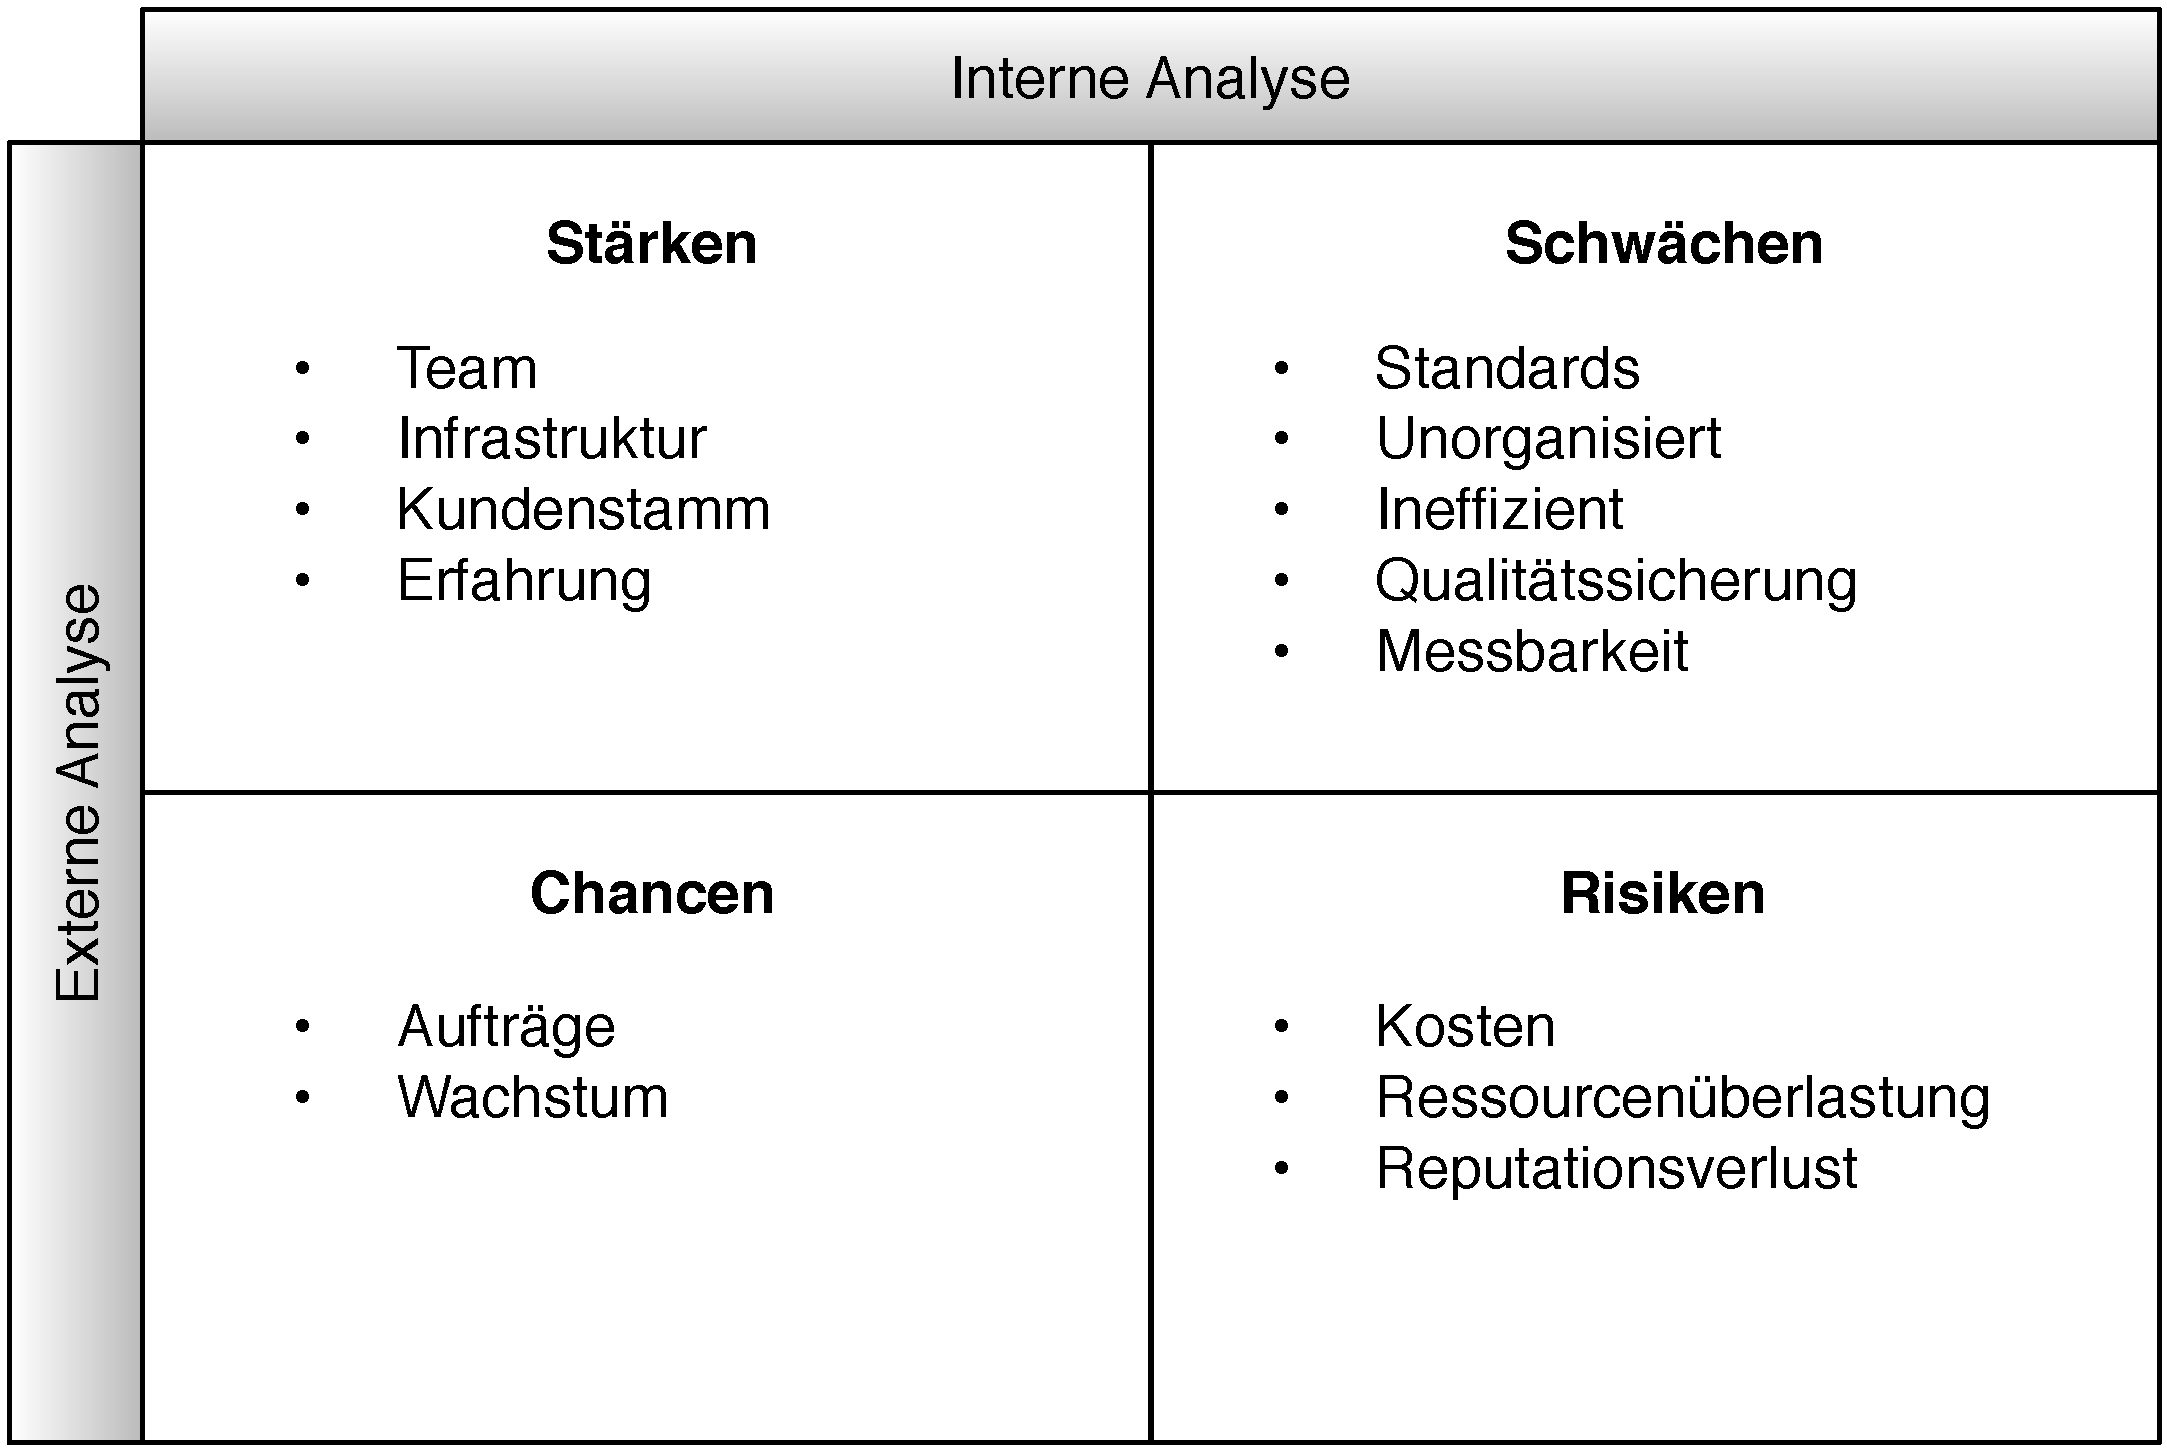
\includegraphics[width=0.8\textwidth,angle=0]{./bilder/analyse/swot_analyse.pdf}
\caption{SWOT-Analyse des Projektablaufes von allink}
\label{pic:swot_analyse}
\end{center}
\end{figure}

Es wird nun im Detail auf die einzelnen Punkte aus der SWOT-Analyse eingegangen
und wo möglich mit einem Beispiel aus der Praxis untermalt.

% Die Ressourcenüberbelastung ist nur ein Problem, das zum Vorschein kommt. In der
% Abbildung \ref{pic:voruntersuchung_projektablauf} verschaffe ich mir einen 
% Überblick über die möglichen Gefahren und Schwächen des aktuellen Projektablaufes.
% 
% \begin{figure}[htbp]
% \begin{center}
% 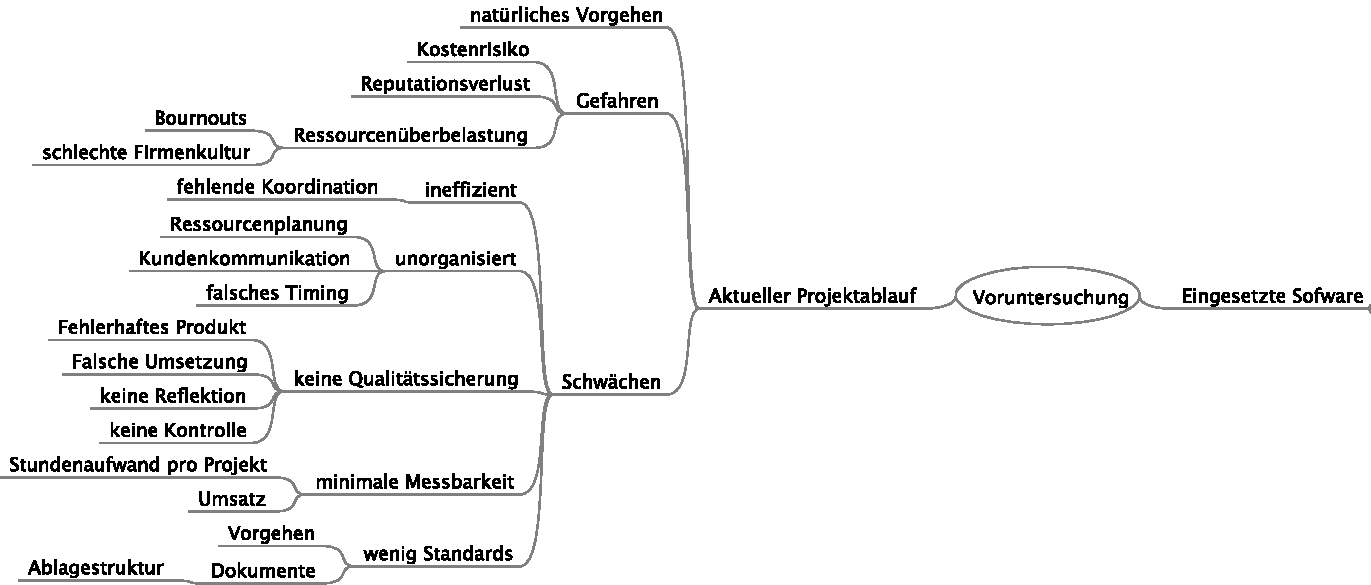
\includegraphics[width=0.95\textwidth,angle=0]{./bilder/analyse/mindmaps/voruntersuchung_projektablauf.pdf}
% \caption{MindMap Voruntersuchung des aktuellen Projektablaufes}
% \label{pic:voruntersuchung_projektablauf}
% \end{center}
% \end{figure}

\subsubsection{Wenig Standards}
Man hält vor, während und nach einem Projekt nur an wenige Standards fest. 
Das ganze Vorgehen ist nicht einheitlich, da in jedem Projekt wieder von
neuem entschieden wird, wie man vorgehen will. Es werden nur wenige einheitlichen
Dokumente verwendet, zum Beispiel für die Erstellung von Offerten und Rechnungen.
Aber auch da entstehen schnell Fehler, z.B. während der Umstellungen des 
Mehrwert Steuersatzes von 7.6\% auf 8\%. Da kein einheitliches Basistemplate
existiert, muss jeder der eine Rechnung schreibt noch einmal sicherstellen, ob
auch der korrekte Steuersatz hinterlegt ist. 

\subsubsection{Unorganisiert}
Durch die Überbelastung können mit der Zeit die versprochenen Timings
nicht mehr eingehalten werden. Da die Ablagestrukturen nicht einheitlich geregelt
sind, kann es vorkommen, dass ein Mitarbeiter einem Kunden ein veraltetes oder
noch nicht freigegebenes Dokument sendet. Dies zieht einen zusätzlichen 
Mehraufwand mit sich, da man sich beim Kunden entschuldigen und rechtfertigen
muss. Zusätzlich strapaziert es auch die Beziehung zum Kunden.

\subsubsection{Ineffizient}
Einfache Abläufe werden so unnötig verkompliziert und aufgehalten. Die ganze
Struktur wird langsam und ineffizient. Was sich wiederum negativ auf die zur
Verfügung stehende Zeit auswirkt.

\subsubsection{Keine Qualitätssicherung}
Oft bleibt gegen Ende eines Projektes dann zu wenig Zeit die nötige 
Qualitätskontrollen durchzuführen, da man sich möglichst schnell um ein anderes,
möglicherweise auch schon überfälliges, Projekt kümmern muss. Der Kunde entdeckt
dann offensichtliche Fehler selbst und zweifelt zwangsläufig an der ganzen Arbeit.

\subsubsection{Minimale Messbarkeit}
Auch bietet die fehlende bzw. chaotische Struktur nur wenige Punkte um Kennzahlen
zu messen. Den Umsatz den man mit dem Projekt erzielt hat ist zwar bekannt,
jedoch kann nur aus dem Gefühl heraus erahnt werden, ob mit dem Projekt einen
Gewinn für die Firma erzielt werden konnte. Die Mitarbeiter sind zwar angehalten
ihre Stunden in ein gemeinsames Stundelog pro Projekt einzutragen, jedoch werden
die Informationen nicht ausgewertet und können nicht mehr einzelnen Mitarbeitern
zugeordnet werden.

\subsubsection{Kostenrisiko}
Durch die fehlende Kontrolle während eines Projektes, verliert man die
Übersicht über die Aufwände und schlussendlich die Kosten. Dadurch entsteht
ein Kostenrisiko, welches Konsequenzen für die Liquidität von allink haben könnte.

\subsubsection{Ressourcenüberbelastung}
Die Belastung für den Mitarbeiter wie auch für die Partner ist so über
längere Zeit nicht tragbar. Durch eine Überarbeitung kann es zu Ausfällen kommen, die
die Situation zusätzlich verschlimmern könnten. Das ganze Endet in einer 
schlechten Firmenkultur und das Unternehmung beginnt von innen zu zerfallen.

\subsubsection{Reputationsverlust}
Da man Timings nicht mehr einhalten kann und man sich gegenüber dem Kunden
oft rechtfertigen muss entsteht ein schlechtes Bild der Unternehmung und sie
verliert an Vertrauen. Da die Konkurrenz im Tätigkeitsfeld der allink relativ
gross ist, ist ein möglicher Absprung und Angenturwechsel seitens des Kunden nicht 
auszuschliessen.
